\chapter{Teori Laju Reaksi}\label{ch:b3:rate-theories}

Pada tahun 2017 disetujui sebuah obat yang satu-satunya perbedaannya dari obat
yang lebih lama adalah bahwa keenam atom hidrogen pada kedua gugus metoksinya
merupakan atom deuterium. Hati menguraikan obat itu dengan memutus tepat
ikatan-ikatan C--H tersebut, dan ikatan C--D terputus beberapa kali lebih
lambat: molekul yang berat itu tinggal lebih lama dalam darah, dan diminum
dalam dosis yang lebih kecil dan lebih jarang. Tidak ada apa pun dalam hukum
Arrhenius yang menjelaskan mengapa sebuah neutron di dalam inti seharusnya
memperlambat suatu reaksi. Bab ini menurunkan tetapan laju dari sifat-sifat
molekul: mula-mula dari tumbukan, lalu dari bentuk \omterm{def:b3:computational-chemistry:pes}{permukaan energi potensial}
dan fungsi-fungsi partisi \omterm{def:b3:rate-theories:tst}{teori keadaan transisi}, yang meramalkan besarnya
efek isotop semacam itu; bab ini diakhiri dengan reaksi dalam larutan, tempat
pelarut menetapkan batas kecepatan.

\begin{recall}
Jilid Tahun 1 mendefinisikan tetapan laju, hukum Arrhenius $k =
A\eu^{-E_a/RT}$ dengan energi aktivasi dan faktor praeksponensialnya, tahap-tahap
elementer, keadaan transisi, profil energi sepanjang koordinat reaksi, dan
postulat Hammond. Jilid Tahun 2 mendefinisikan kekuatan ion dan koefisien
aktivitas, dengan hukum pembatas Debye--Hückel $\log\gamma_i = -Az_i^2\sqrt I$ ($A \approx
0.51$ dalam air pada \qty{25}{\celsius}), serta mencocokkan garis kuadrat terkecil.
\Cref{ch:b3:computational-chemistry} memperkenalkan \omterm{def:b3:computational-chemistry:pes}{permukaan energi potensial};
\cref{ch:b3:partition-functions,ch:b3:statistical-thermo-applied} menghitung
tetapan kesetimbangan dari fungsi partisi dan \omterm{def:b3:quantum-model-systems:oscillator}{energi titik nol}. Dari fisika:
distribusi Maxwell--Boltzmann kelajuan molekul, dan hukum difusi Fick.
\end{recall}

\begin{omfigure}
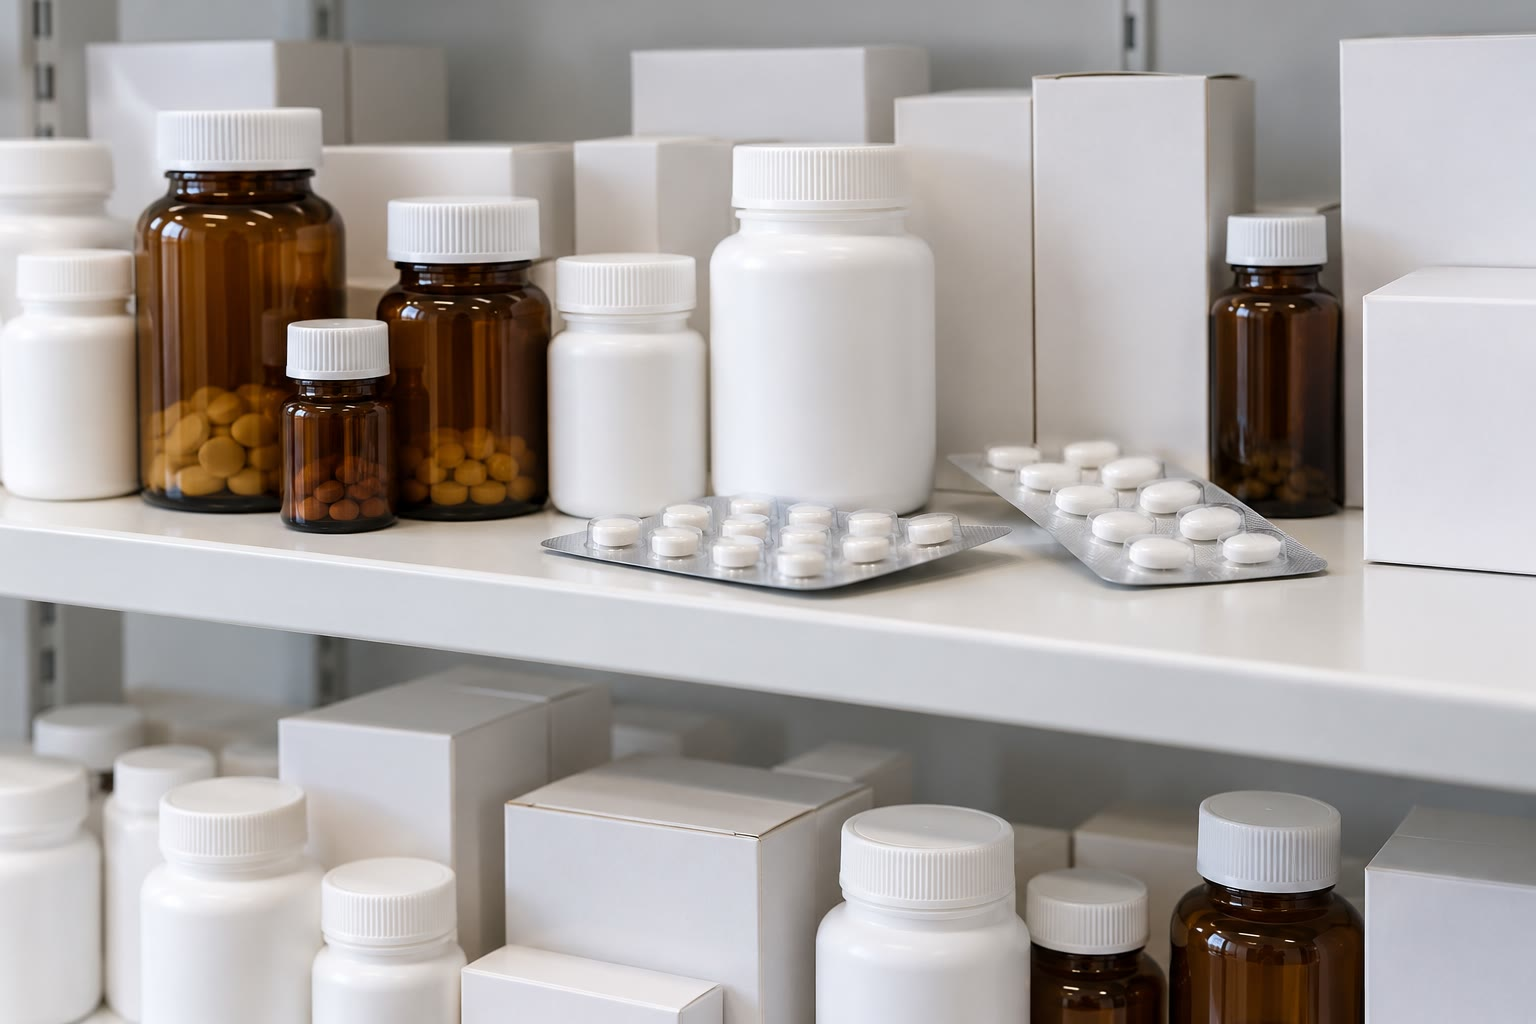
\includegraphics[width=0.6\linewidth]{images/book4/ai/b3-12-pharmacy.jpg}

{\small Obat-obatan di rak apotek. Mengganti hidrogen dengan deuterium pada
ikatan-ikatan yang pertama kali diserang hati dapat memperpanjang waktu obat
tinggal di dalam tubuh.}
\end{omfigure}

\section{Teori tumbukan}

Dua molekul dalam gas hanya dapat bereaksi jika keduanya bertemu. Modelkan
keduanya sebagai bola keras berdiameter $d_{\mathrm A}$ dan $d_{\mathrm B}$: keduanya
bertumbukan ketika pusat-pusatnya lewat dalam jarak $d =
\frac12(d_{\mathrm A} + d_{\mathrm B})$ satu sama lain.

\begin{definition}[Penampang tumbukan, faktor sterik]\label{def:b3:rate-theories:collision}
Yang disebut \emph{penampang tumbukan}\index{penampang tumbukan} dua molekul
adalah luas $\sigma = \pi d^2$ cakram, yang tegak lurus pada kecepatan
relatifnya, yang harus dilewati pusat satu molekul agar mengenai molekul yang
lain. Yang disebut \emph{faktor sterik}\index{faktor sterik} $P$ adalah rasio
faktor praeksponensial terukur sebuah reaksi terhadap faktor yang diramalkan
oleh teori tumbukan.
\end{definition}

\begin{omfigure}
\begin{tikzpicture}[font=\small, >=Stealth]
  \shade[ball color=omDef!40] (0,0) circle (0.45);
  \node at (0,0) {A};
  \draw[black!50, dashed] (-0.0,0.85) -- (5.2,0.85) (-0.0,-0.85) -- (5.2,-0.85);
  \draw[black!60] (0,0) ellipse (0.25 and 0.85);
  \draw[<->] (-0.45,0) -- (-0.45,0.85) node[midway, left] {$d$};
  \shade[ball color=omThm!40] (3.3,0.55) circle (0.4);
  \node at (3.3,0.55) {B};
  \shade[ball color=omThm!20] (4.6,1.45) circle (0.4);
  \node at (4.6,1.45) {B};
  \draw[->, thick] (0.6,0) -- (2.2,0) node[midway, below] {$v_{\mathrm{rel}}\,\Delta t$};
  \node[anchor=west, align=left, font=\scriptsize] at (5.3,0) {silinder\\ berpenampang\\ $\sigma = \pi d^2$};
  \node[font=\scriptsize, anchor=south] at (3.3,1.0) {kena};
  \node[font=\scriptsize, anchor=south] at (4.6,1.9) {luput};
\end{tikzpicture}

{\small Silinder tumbukan. Dengan bergerak pada kelajuan relatif $v_{\mathrm{rel}}$,
molekul A menyapu dalam waktu $\Delta t$ sebuah silinder berpenampang
$\sigma = \pi d^2$, dengan $d$ jumlah kedua jari-jarinya; setiap B yang pusatnya
berada di dalamnya terkena.}
\end{omfigure}

\begin{theorem}[Tetapan laju menurut teori tumbukan]\label{thm:b3:rate-theories:collision}
Jika setiap tumbukan yang energi kinetiknya sepanjang garis pusat melebihi
ambang $E_0$ (per mol) menghasilkan reaksi, maka tetapan laju
$\mathrm{A + B} \to$ produk adalah
\[
  k = \sigma\bar v_{\mathrm{rel}}N_A\,\eu^{-E_0/RT}, \qquad \bar v_{\mathrm{rel}} = \sqrt{\frac{8kT}{\pi\mu}},\
  \mu = \frac{m_{\mathrm A}m_{\mathrm B}}{m_{\mathrm A} + m_{\mathrm B}} .
\]
\end{theorem}

\begin{proof}[Bukti parsial]
Dalam waktu $\Delta t$, sebuah molekul A menyapu volume $\sigma v_{\mathrm{rel}}\Delta t$ dan
mengenai $n_{\mathrm B}\sigma v_{\mathrm{rel}}\Delta t$ molekul B yang dimuatnya: laju tumbukan per
satuan volume adalah $\sigma\bar v_{\mathrm{rel}}n_{\mathrm A}n_{\mathrm B}$, dengan $\bar v_{\mathrm{rel}}$
kelajuan relatif rata-rata yang diberikan oleh distribusi Maxwell--Boltzmann
(diterima dari fisika, dengan \omterm{def:b3:quantum-model-systems:oscillator}{massa tereduksi}). Memberi bobot setiap tumbukan
menurut kelajuannya dan mempertahankan tumbukan-tumbukan yang energinya
sepanjang garis pusat melebihi ambang menyisakan fraksi $\eu^{-E_0/RT}$ dari laju
tumbukan (integrasi atas parameter tumbukan diterima tanpa bukti). Mengubah
kerapatan jumlah menjadi konsentrasi molar mengalikannya dengan $N_A$.
\end{proof}

Karena $\bar v_{\mathrm{rel}} \propto \sqrt T$, energi aktivasinya $E_a = RT^2\,\dd\ln k/\dd T$ adalah
$E_0 + \frac12RT$, dekat dengan ambangnya. Faktor praeksponensialnya berorde
$10^{11}$~\unit{L.mol^{-1}.s^{-1}} untuk molekul kecil. Faktor yang terukur sering
jauh lebih kecil: $P \ll 1$ untuk molekul yang harus bertemu dalam orientasi
tertentu, dan \omterm{def:b3:rate-theories:collision}{penampang tumbukan} tidak mempunyai nilai tunggal untuk
molekul-molekul nyata, yang bukan bola keras. Teori tumbukan memberikan orde
besaran dan ketergantungan pada suhu; teori itu tidak dapat memberikan
$E_0$, yang memerlukan \omterm{def:b3:computational-chemistry:pes}{permukaan energi potensial}.

\section{Permukaan energi potensial}

Reaksi $\mathrm{H_A + H_BH_C \to H_AH_B + H_C}$ adalah reaksi yang paling sederhana. Untuk
pendekatan kolinear, energinya bergantung pada dua jarak, $r_{\mathrm{AB}}$ dan
$r_{\mathrm{BC}}$, dan dapat digambar sebagai peta.

\begin{definition}[Titik pelana, lintasan energi minimum]\label{def:b3:rate-theories:saddle}
Yang disebut \emph{titik pelana}\index{titik pelana} \omterm{def:b3:computational-chemistry:pes}{permukaan energi potensial}
adalah titik tempat gradien lenyap, energi maksimum sepanjang satu arah dan
minimum sepanjang semua arah lainnya. Yang disebut \emph{lintasan energi
minimum}\index{lintasan energi minimum} adalah lintasan penurunan tercuram
dari titik pelana ke lembah pereaksi dan lembah produk; panjangnya yang diukur
sepanjang lintasan itu adalah koordinat reaksi, dan titik pelana itu adalah
keadaan transisi.
\end{definition}

\begin{omfigure}
\begin{tikzpicture}
\begin{axis}[ompes, width=0.62\linewidth, xmin=0.4, xmax=3.0, ymin=0.4, ymax=3.0,
  xlabel={$r_{\mathrm{AB}}$ / \AA}, ylabel={$r_{\mathrm{BC}}$ / \AA},
  colorbar, colorbar style={ylabel={$E$ / eV}, ylabel style={font=\small},
  yticklabel style={font=\small}}, point meta min=-4.7, point meta max=-0.8]
\addplot3[contour prepared={labels=false}, thick] table {figdata/out/bachelor-3-pes-collinear-contours.dat};
\addplot3[ompath] table[x=x, y=y, z expr=0] {figdata/out/bachelor-3-pes-collinear-mep.dat};
\node[omsaddle] at (axis cs:0.918,0.918,0) {};
\node[font=\small, anchor=south west] at (axis cs:0.95,0.95,0) {pelana};
\node[font=\small, anchor=west, fill=white, fill opacity=0.85, text opacity=1, inner sep=1.5pt] at (axis cs:2.05,1.0,0) {$\mathrm{H_A + H_BH_C}$};
\node[font=\small, anchor=west, fill=white, fill opacity=0.85, text opacity=1, inner sep=1.5pt] at (axis cs:0.95,2.55,0) {$\mathrm{H_AH_B + H_C}$};
\node[font=\small, anchor=north east] at (axis cs:2.95,2.95,0) {$\ce{H + H + H}$};
\end{axis}
\end{tikzpicture}

{\small Model \omterm{def:b3:computational-chemistry:pes}{permukaan energi potensial} untuk $\ce{H + H2}$ kolinear (bentuk LEPS
yang dibangun dari kurva Morse \ce{H2}, dengan parameter Sato 0.17 yang dipilih
sebagai tetapan model). Kontur dari \qty{-4.65}{eV} sampai \qty{-0.8}{eV}, dengan
energi nol untuk tiga atom yang terpisah; lembah-lembahnya terletak pada
\qty{-4.75}{eV}, kedalaman sumur \ce{H2}. Garis putus-putus: \omterm{def:b3:rate-theories:saddle}{lintasan energi
minimum}, yang melintasi pelana simetris pada $r_{\mathrm{AB}} = r_{\mathrm{BC}} = \qty{0.92}{\angstrom}$,
\qty{0.27}{eV} di atas lembah-lembah dalam model ini.}
\end{omfigure}

Lintasan itu mendaki keluar dari lembah pereaksi, tempat $r_{\mathrm{BC}}$ tetap
dekat dengan panjang ikatan \ce{H2} sementara A mendekat, melintasi pelana, lalu
turun ke lembah produk. Di pelana, kedua ikatan teregang sampai
\qty{0.92}{\angstrom}: ikatan lama setengah putus dan ikatan baru setengah
terbentuk, dan biaya energi kompromi inilah penghalangnya. Untuk reaksi
simetris, pelananya terletak pada diagonal; untuk reaksi eksoterm, pelana itu
bergeser ke arah lembah pereaksi (penghalang awal, keadaan transisi yang mirip
pereaksi, seperti dinyatakan postulat Hammond), dan untuk reaksi endoterm ke
arah lembah produk (penghalang akhir). Posisinya menentukan energi mana yang
membantu: energi translasi, yang terarah sepanjang lembah masuk, membawa
molekul-molekul melewati penghalang awal; penghalang akhir, yang terletak di
balik tikungan, lebih mudah dilewati dengan energi vibrasi pada ikatan yang
putus. Inilah aturan-aturan Polanyi, yang dikukuhkan oleh eksperimen berkas
molekul.

\section{Teori keadaan transisi}

\begin{definition}[Kompleks teraktivasi]\label{def:b3:rate-theories:activated-complex}
Yang disebut \emph{kompleks teraktivasi}\index{kompleks teraktivasi} sebuah
tahap elementer adalah himpunan konfigurasi sistem yang bereaksi dalam irisan
tipis di sekitar \omterm{def:b3:rate-theories:saddle}{titik pelana}, yang tegak lurus pada \omterm{def:b3:rate-theories:saddle}{lintasan energi minimum};
kompleks itu diperlakukan sebagai spesies $\ce{AB^{\ddagger}}$, dengan fungsi
partisinya sendiri.
\end{definition}

\begin{definition}[Teori keadaan transisi, koefisien transmisi]\label{def:b3:rate-theories:tst}
Yang disebut \emph{teori keadaan transisi}\index{teori keadaan transisi} adalah
teori yang menganggap bahwa \omterm{def:b3:rate-theories:activated-complex}{kompleks-kompleks teraktivasi} berada dalam
kesetimbangan dengan pereaksi, bahwa setiap kompleks yang melintasi daerah
pelana ke arah produk terus membentuk produk itu, dan bahwa gerak sepanjang
koordinat reaksi adalah translasi bebas. Yang disebut \emph{koefisien
transmisi}\index{koefisien transmisi} $\kappa \le 1$ mengoreksi kompleks-kompleks
yang melintas kembali ke pereaksi.
\end{definition}

\begin{theorem}[Persamaan Eyring]\label{thm:b3:rate-theories:eyring}
Untuk tahap elementer $\mathrm{A + B} \to \mathrm{AB}^{\ddagger} \to$ produk,
\[
  k = \kappa\frac{k_BT}{h}\overline{K}{}^{\ddagger}, \qquad
  \overline{K}{}^{\ddagger} = \frac{\bar q^{\ddagger}/N_A}{(q_{\mathrm A}/N_A)(q_{\mathrm B}/N_A)}\,\eu^{-\Delta E_0^{\ddagger}/RT},
\]
dengan $\bar q^{\ddagger}$ fungsi partisi \omterm{def:b3:rate-theories:activated-complex}{kompleks teraktivasi} tanpa gerak koordinat
reaksi, $q$ fungsi partisi molar per satuan volume, dan $\Delta E_0^{\ddagger}$ tinggi
tingkat titik nol kompleks itu di atas tingkat titik nol pereaksi. Dalam
bentuk termodinamika, dengan $c^\circ = \qty{1}{mol/L}$ dan molekularitas $m$,
\[
  k = \kappa\frac{k_BT}{h}(c^\circ)^{1-m}\,\eu^{\Delta^{\ddagger}S^\circ/R}\,\eu^{-\Delta^{\ddagger}H^\circ/RT}.
\]
Pernyataan ini disebut \emph{persamaan Eyring}\index{persamaan Eyring}; $k_B$
adalah tetapan Boltzmann, yang ditulis demikian agar tidak tertukar dengan $k$.
\end{theorem}

\begin{proof}
Kesetimbangan semu: $[\ce{AB^{\ddagger}}] = K^{\ddagger}[\mathrm A][\mathrm B]$, dengan $K^{\ddagger}$
dari fungsi-fungsi partisi
(\cref{thm:b3:statistical-thermo-applied:k-from-q}, yang ditulis dengan
konsentrasi). Dari vibrasi-vibrasi kompleks itu, satu adalah gerak sepanjang
koordinat reaksi: vibrasi yang sangat longgar dengan frekuensi
$\nu \ll k_BT/h$, yang fungsi partisinya $k_BT/h\nu$ (limit suhu tinggi
\cref{prop:b3:partition-functions:q-vib}); jadi $q^{\ddagger} = \bar q^{\ddagger}k_BT/h\nu$.
Kompleks-kompleks itu melintas ke arah produk dengan frekuensi $\nu$ gerak ini,
sehingga lajunya adalah $\nu[\ce{AB^{\ddagger}}] = \nu\frac{k_BT}{h\nu}\overline{K}{}^{\ddagger}[\mathrm A][\mathrm B]$:
$\nu$ yang tidak diketahui saling meniadakan. Menuliskan
$\overline{K}{}^{\ddagger} = (c^\circ)^{1-m}\eu^{-\Delta^{\ddagger}G^\circ/RT}$ dan
$\Delta^{\ddagger}G^\circ = \Delta^{\ddagger}H^\circ - T\Delta^{\ddagger}S^\circ$ memberikan bentuk
kedua, dengan $\kappa$ disisipkan untuk lintasan balik.
\end{proof}

Faktor $k_BT/h$ bernilai \qty{6.2e12}{s^{-1}} pada \qty{298}{K}: laju tahap
unimolekuler tanpa penghalang dan tanpa kehilangan entropi. Segala sesuatu
yang khas bagi reaksi itu terletak dalam besaran-besaran aktivasi.

\begin{definition}[Energi Gibbs, entalpi, dan entropi aktivasi]\label{def:b3:rate-theories:activation}
Yang disebut \emph{energi Gibbs aktivasi}\index{energi Gibbs aktivasi}
$\Delta^{\ddagger}G^\circ$, \emph{entalpi aktivasi}\index{entalpi aktivasi}
$\Delta^{\ddagger}H^\circ$, dan \emph{entropi aktivasi}\index{entropi aktivasi}
$\Delta^{\ddagger}S^\circ$ sebuah tahap elementer adalah energi Gibbs, entalpi,
dan entropi standar pembentukan \omterm{def:b3:rate-theories:activated-complex}{kompleks teraktivasi} (tanpa gerak koordinat
reaksinya) dari pereaksi, yang didefinisikan oleh \omterm{thm:b3:rate-theories:eyring}{persamaan Eyring}.
\end{definition}

\begin{proposition}[Energi aktivasi dan entalpi aktivasi]\label{prop:b3:rate-theories:ea-dh}
Untuk reaksi dalam larutan, $E_a = \Delta^{\ddagger}H^\circ + RT$; untuk reaksi gas
bimolekuler, $E_a = \Delta^{\ddagger}H^\circ + 2RT$.
\end{proposition}

\begin{proof}
$E_a = RT^2\,\dd\ln k/\dd T$, dan $\ln k = \ln T + \Delta^{\ddagger}S^\circ/R - \Delta^{\ddagger}H^\circ/RT + $ tetapan: $E_a =
RT + \Delta^{\ddagger}H^\circ$ jika parameter aktivasi tidak berubah terhadap $T$. Dalam
larutan, inilah hasilnya. Dalam fase gas, hubungan van 't Hoff untuk
$K^{\ddagger}$ yang ditulis dalam konsentrasi melibatkan energi dalam,
$\Delta^{\ddagger}U^\circ = \Delta^{\ddagger}H^\circ - \Delta n^{\ddagger}RT$
dengan $\Delta n^{\ddagger} = 1 - m$: untuk $m = 2$, $E_a = \Delta^{\ddagger}H^\circ + 2RT$.
\end{proof}

\omterm{def:b3:rate-theories:activation}{Entropi aktivasi} membaca struktur keadaan transisi. Dua molekul yang bergabung
menjadi satu kompleks kehilangan kebebasan translasi dan rotasi:
$\Delta^{\ddagger}S^\circ$ sangat negatif, $-50$ sampai $-150$ \unit{J.K^{-1}.mol^{-1}}, untuk
tahap-tahap asosiatif dan keadaan transisi siklik. Molekul yang melonggarkan
sebuah ikatan dalam perjalanannya menuju disosiasi memperoleh kebebasan:
$\Delta^{\ddagger}S^\circ > 0$.

\begin{proposition}[Galat baku garis yang dicocokkan]\label{prop:b3:rate-theories:slope-uncertainty}
Untuk garis kuadrat terkecil $y = a + bx$ melalui $n$ titik yang nilai $y$-nya
mengandung galat saling bebas dengan variansi yang sama, yang ditaksir dengan
$s^2 = \sum_i(y_i - a - bx_i)^2/(n - 2)$, kemiringan dan perpotongannya
mempunyai galat baku
\[
  s_b = \frac{s}{\sqrt{\sum_i(x_i - \bar x)^2}}, \qquad
  s_a = s\sqrt{\frac1n + \frac{\bar x^2}{\sum_i(x_i - \bar x)^2}} .
\]
\end{proposition}

\begin{proof}
$b = \sum_i(x_i - \bar x)y_i/S_{xx}$, dengan $S_{xx} = \sum_i(x_i - \bar x)^2$, adalah
kombinasi linear $y_i$ yang saling bebas dengan variansi $\sigma^2$: variansinya
adalah $\sigma^2\sum_i(x_i - \bar x)^2/S_{xx}^2 = \sigma^2/S_{xx}$. Demikian pula
$a = \bar y - b\bar x$, dan $\bar y$ serta $b$ tidak berkorelasi (kovariansinya
$\sigma^2\sum_i(x_i - \bar x)/(nS_{xx}) = 0$), sehingga
$\operatorname{var}a = \sigma^2/n + \bar x^2\sigma^2/S_{xx}$. Mengganti $\sigma^2$
dengan taksirannya $s^2$ (pembagi $n - 2$ memperhitungkan kedua parameter yang
dicocokkan, diterima tanpa bukti) memberikan hasilnya.
\end{proof}

\begin{method}[Grafik Eyring dengan ketidakpastiannya]\label{met:b3:rate-theories:eyring-plot}
\begin{enumerate}
  \item Ukurlah $k$ pada lima suhu atau lebih yang tersebar dalam rentang 30
        sampai \qty{40}{K}.
  \item Alurkan $y = \ln(k/T)$ terhadap $x = 1/T$ dan cocokkan garis kuadrat
        terkecil $y = a + bx$.
  \item $\Delta^{\ddagger}H^\circ = -Rb$ dan $\Delta^{\ddagger}S^\circ = R[a - \ln(k_B/h)]$
        ($\ln(k_B/h) = 23.760$ dengan $k$ dalam \unit{s^{-1}}).
  \item Galat bakunya adalah $Rs_b$ dan $Rs_a$; selang kepercayaan 95\,\%
        mengalikannya dengan $t$ Student untuk $n - 2$ derajat kebebasan
        (3.18 untuk lima titik).
  \item Perpotongan terletak jauh di luar rentang yang diukur, pada
        $1/T = 0$: $\Delta^{\ddagger}S^\circ$ selalu jauh kurang presisi daripada
        $\Delta^{\ddagger}H^\circ$, dan galat keduanya berkorelasi.
\end{enumerate}
\end{method}

\begin{omfigure}
\begin{tikzpicture}
\begin{axis}[width=0.74\linewidth, height=6.2cm, xmin=3.12, xmax=3.62, ymin=-12.8, ymax=-6.4,
  axis lines=left, xlabel={$1000\,\mathrm K/T$}, ylabel={$\ln\bigl(k/(\mathrm s^{-1}\,\mathrm K^{-1})\bigr)$},
  tick label style={font=\small}, label style={font=\small},
  legend style={font=\scriptsize, draw=none, fill=white, fill opacity=0.85, text opacity=1,
  at={(0.98,0.98)}, anchor=north east}, legend cell align=left]
\addplot[omDef, thick] table[x=invT, y=fit] {figdata/out/bachelor-3-eyring-band-H.dat};
\addplot[omThm, thick] table[x=invT, y=fit] {figdata/out/bachelor-3-eyring-band-D.dat};
\addplot[omDef, thin, dashed, forget plot] table[x=invT, y=lo] {figdata/out/bachelor-3-eyring-band-H.dat};
\addplot[omDef, thin, dashed, forget plot] table[x=invT, y=hi] {figdata/out/bachelor-3-eyring-band-H.dat};
\addplot[omThm, thin, dashed, forget plot] table[x=invT, y=lo] {figdata/out/bachelor-3-eyring-band-D.dat};
\addplot[omThm, thin, dashed, forget plot] table[x=invT, y=hi] {figdata/out/bachelor-3-eyring-band-D.dat};
\addplot[only marks, mark=*, mark size=1.8pt, omDef, forget plot] table[x=invT, y=lnkT_H] {figdata/out/bachelor-3-eyring-points.dat};
\addplot[only marks, mark=square*, mark size=1.7pt, omThm, forget plot] table[x=invT, y=lnkT_D] {figdata/out/bachelor-3-eyring-points.dat};
\legend{obat \ce{OCH3}, obat \ce{OCD3}}
\end{axis}
\end{tikzpicture}

{\small Grafik Eyring tetapan-tetapan laju soal akhir pekan (data soal) untuk
obat itu dan analognya yang terdeuterasi, dengan garis-garis kuadrat terkecil
beserta pita kepercayaan 95\,\% (garis putus-putus, hampir tidak lebih lebar
daripada garisnya: titik-titiknya tersebar sekitar 1\,\%). Kedua garis sejajar
dalam batas ketidakpastiannya: \omterm{def:b3:rate-theories:activation}{entropi aktivasinya} sama, \omterm{def:b3:rate-theories:activation}{entalpi aktivasinya}
berbeda sekitar \qty{5}{kJ/mol}.}
\end{omfigure}

\section{Efek isotop kinetik}

\begin{definition}[Efek isotop kinetik]\label{def:b3:rate-theories:kie}
Yang disebut \emph{efek isotop kinetik}\index{efek isotop kinetik} sebuah tahap
adalah rasio $k_{\mathrm{ringan}}/k_{\mathrm{berat}}$ tetapan-tetapan lajunya untuk dua
\omterm{def:b3:rovibrational-spectroscopy:rotational-constant}{isotopolog}, paling sering $k_{\mathrm H}/k_{\mathrm D}$. Efek itu disebut
\emph{efek isotop kinetik primer}\index{efek isotop kinetik primer} jika ikatan
ke atom yang disubstitusi terbentuk atau putus dalam tahap itu, dan
\emph{efek isotop kinetik sekunder}\index{efek isotop kinetik sekunder} jika
tidak.
\end{definition}

\begin{proposition}[Efek isotop kinetik primer maksimum]\label{prop:b3:rate-theories:primary-kie}
Jika vibrasi ulur ikatan X--H menjadi koordinat reaksi, sehingga \omterm{def:b3:quantum-model-systems:oscillator}{energi titik
nolnya} hilang dalam keadaan transisi sementara semua sumbangan lain sama untuk
H dan D,
\[
  \frac{k_{\mathrm H}}{k_{\mathrm D}} = \exp\Bigl[\frac{hc(\tilde\nu_{\mathrm{XH}} - \tilde\nu_{\mathrm{XD}})}{2k_BT}\Bigr],
  \qquad \frac{\tilde\nu_{\mathrm{XH}}}{\tilde\nu_{\mathrm{XD}}} = \sqrt{\frac{\mu_{\mathrm{XD}}}{\mu_{\mathrm{XH}}}} .
\]
\end{proposition}

\begin{proof}
\omterm{def:b3:computational-chemistry:pes}{Permukaan energi potensialnya} sama untuk kedua \omterm{def:b3:rovibrational-spectroscopy:rotational-constant}{isotopolog} (elektron-elektron
tidak melihat neutron). Dalam pereaksi, vibrasi ulur X--H menyimpan
$\frac12hc\tilde\nu_{\mathrm{XH}}$ \omterm{def:b3:quantum-model-systems:oscillator}{energi titik nol}; dalam keadaan transisi modus ini telah
menjadi koordinat reaksi dan tidak menyimpan apa pun. Oleh karena itu,
penghalang yang diukur antara tingkat-tingkat titik nol lebih rendah untuk H
sebesar $\frac12hc\tilde\nu_{\mathrm{XH}}$ dan untuk D sebesar $\frac12hc\tilde\nu_{\mathrm{XD}}$:
$\Delta E_0^{\ddagger}(\mathrm D) -
\Delta E_0^{\ddagger}(\mathrm H) = \frac12hc(\tilde\nu_{\mathrm{XH}} - \tilde\nu_{\mathrm{XD}})$, dan \omterm{thm:b3:rate-theories:eyring}{persamaan
Eyring} memberikan rasionya jika faktor-faktor lain saling meniadakan.
Bilangan gelombang sebuah vibrasi ulur sebanding dengan $1/\sqrt\mu$
(\cref{ch:b3:rovibrational-spectroscopy}).
\end{proof}

\begin{omfigure}
\begin{tikzpicture}[font=\small, >=Stealth, x=1cm, y=1cm]
  \draw[->] (-1.4,0) -- (-1.4,4.7) node[anchor=south] {$E$};
  \draw[->] (-1.4,0) -- (10.6,0) node[anchor=north east] {koordinat reaksi};
  \draw[very thick, black!70] plot[smooth, tension=0.6] coordinates {(1.6,3.4) (2.1,1.6) (2.7,0.8)
    (3.3,0.6) (3.9,0.8) (4.7,2.0) (5.5,3.6) (6.2,4.0) (6.9,3.6) (7.7,2.2) (8.5,1.2) (9.2,1.0)
    (9.9,1.2) (10.4,1.7)};
  \draw[black!50, dashed] (2.8,0.6) -- (3.8,0.6);
  \draw[omDef, thick] (2.42,1.35) -- (4.2,1.35);
  \draw[omThm, thick] (2.5,1.05) -- (4.05,1.05);
  \node[omDef, font=\scriptsize, anchor=south] at (3.3,1.37) {C--H};
  \node[omThm, font=\scriptsize, anchor=north] at (3.3,1.03) {C--D};
  \draw[black, thick] (5.7,4.0) -- (6.7,4.0);
  \draw[black!40, densely dotted] (0.0,4.0) -- (5.7,4.0);
  \draw[black!40, densely dotted] (0.7,1.35) -- (2.42,1.35) (0.0,1.05) -- (2.5,1.05);
  \draw[<->, omThm] (0.0,1.05) -- (0.0,4.0) node[pos=0.5, left, font=\scriptsize] {$E_0(\mathrm D)$};
  \draw[<->, omDef] (0.7,1.35) -- (0.7,4.0) node[pos=0.5, right, font=\scriptsize] {$E_0(\mathrm H)$};
  \node[anchor=south, align=center, font=\scriptsize] at (6.2,4.05) {keadaan transisi: vibrasi ulur itu\\ telah menjadi koordinat reaksi};
\end{tikzpicture}

{\small Asal-usul \omterm{def:b3:rate-theories:kie}{efek isotop kinetik primer}. Dalam pereaksi, vibrasi ulur C--H
menyimpan lebih banyak \omterm{def:b3:quantum-model-systems:oscillator}{energi titik nol} daripada vibrasi ulur C--D
(tingkat-tingkat di atas dasar sumur, garis putus-putus); dalam keadaan
transisi vibrasi ini telah menjadi koordinat reaksi, dan kedua \omterm{def:b3:rovibrational-spectroscopy:rotational-constant}{isotopolog}
mencapai puncak yang sama. Penghalangnya lebih besar untuk D sebesar selisih
\omterm{def:b3:quantum-model-systems:oscillator}{energi titik nol} keduanya.}
\end{omfigure}

\begin{omfigure}
\begin{tikzpicture}
\begin{axis}[width=0.7\linewidth, height=5.6cm, xmin=200, xmax=800, ymin=1, ymax=50,
  ymode=log, axis lines=left, xlabel={$T$ / K}, ylabel={$k_{\mathrm H}/k_{\mathrm D}$ (maksimum)},
  tick label style={font=\small}, label style={font=\small}, log ticks with fixed point,
  ytick={1,2,5,10,20,50}, legend style={font=\scriptsize, draw=none, at={(0.98,0.98)},
  anchor=north east}, legend cell align=left]
\addplot[omThm, thick] table[x=T, y=OH] {figdata/out/bachelor-3-kie.dat};
\addplot[black!60, thick] table[x=T, y=NH] {figdata/out/bachelor-3-kie.dat};
\addplot[omDef, thick] table[x=T, y=CH] {figdata/out/bachelor-3-kie.dat};
\legend{O--H (\qty{3657}{cm^{-1}}), N--H (\qty{3337}{cm^{-1}}), C--H (\qty{2917}{cm^{-1}})}
\end{axis}
\end{tikzpicture}

{\small \omterm{def:b3:rate-theories:kie}{Efek isotop kinetik primer} maksimum terhadap suhu untuk hilangnya
vibrasi ulur C--H, N--H, atau O--H (fundamental \ce{CH4}, \ce{NH3} dan \ce{H2O};
bilangan gelombang deuterium dari \omterm{def:b3:quantum-model-systems:oscillator}{massa tereduksinya}). Pada \qty{298}{K}
nilainya 6.5 untuk C--H; nilai itu menurun menuju 1 ketika suhu naik.}
\end{omfigure}

Nilai maksimum C--H pada suhu kamar, sekitar 7, adalah sebuah tolok ukur. Efek
teramati sebesar 2 sampai 7 menunjukkan bahwa ikatan C--H putus dalam tahap
penentu laju; nilai yang lebih kecil menunjukkan bahwa keadaan transisi
mempertahankan sebagian vibrasi ulur itu (transfer hidrogen yang asimetris,
awal, atau akhir), atau bahwa tahap itu bukan tahap yang paling lambat. Nilai
yang jauh lebih besar daripada 7 pada suhu kamar tidak mungkin berasal dari
\omterm{def:b3:quantum-model-systems:oscillator}{energi titik nol}: nilai itu mengungkap \omterm{def:b3:quantum-model-systems:tunnelling}{penerowongan}
(\cref{ch:b3:quantum-model-systems}), yang jauh lebih jarang dilakukan partikel
bermassa dua kali lipat. Efek sekunder, yang berasal dari perubahan vibrasi
tekuk ikatan-ikatan C--H di sebelah pusat yang bereaksi, kecil, biasanya 0.8
sampai 1.2 per deuterium; efek ini membedakan, misalnya, karbon yang menjadi
trigonal (sp$^3$ ke sp$^2$, $k_{\mathrm H}/k_{\mathrm D} > 1$) dari karbon yang menjadi
tetrahedral ($< 1$).

\begin{method}[Mengukur efek isotop kinetik dengan kompetisi]\label{met:b3:rate-theories:kie}
\begin{enumerate}
  \item Jalankan reaksi pada campuran kedua \omterm{def:b3:rovibrational-spectroscopy:rotational-constant}{isotopolog}, atau pada molekul yang
        membawa H pada satu posisi dan D pada posisi yang ekuivalen.
  \item Hentikan pada konversi rendah dan ukurlah rasio produk H dan D dengan
        spektrometri massa atau NMR.
  \item Rasio produk, yang dikoreksi terhadap rasio awal, adalah
        $k_{\mathrm H}/k_{\mathrm D}$; kedua \omterm{def:b3:rovibrational-spectroscopy:rotational-constant}{isotopolog} mengalami kondisi yang tepat sama,
        yang membuat metode ini lebih presisi daripada dua pengukuran laju yang
        terpisah.
\end{enumerate}
\end{method}

\section{Reaksi dalam larutan}

Dalam cairan, sebuah molekul tidak terbang bebas di antara tumbukan: molekul
itu bergetar dalam sangkar tetangga-tetangganya, bertumbukan dengan mereka
berkali-kali sebelum berdifusi menjauh. Dua pereaksi yang bertemu tetap
bersama selama banyak tumbukan, yang disebut sebuah pertemuan.

\begin{definition}[Kendali difusi dan kendali aktivasi, efek sangkar]\label{def:b3:rate-theories:diffusion}
Sebuah reaksi dalam larutan disebut \emph{reaksi terkendali
difusi}\index{reaksi terkendali difusi} jika reaksi pada setiap pertemuan berlangsung cepat,
sehingga lajunya sama dengan laju pereaksi-pereaksi berdifusi saling mendekat;
reaksi itu disebut \emph{reaksi terkendali
aktivasi}\index{reaksi terkendali aktivasi} jika hanya sebagian kecil pertemuan yang menghasilkan reaksi. Yang
disebut \emph{efek sangkar}\index{efek sangkar} adalah terkurungnya sepasang
molekul oleh pelarut di sekitarnya, yang membuat keduanya bertumbukan
berulang-ulang selama satu pertemuan.
\end{definition}

\begin{proposition}[Limit Smoluchowski]\label{prop:b3:rate-theories:smoluchowski}
Tetapan laju \omterm{def:b3:rate-theories:diffusion}{reaksi terkendali difusi} antara bola-bola yang bereaksi pada
jarak $R^*$ adalah $k_d = 4\pi N_A(D_{\mathrm A} + D_{\mathrm B})R^*$. Dengan hubungan
Stokes--Einstein $D = k_BT/6\pi\eta a$ untuk bola berjari-jari $a$ dalam
pelarut berviskositas $\eta$, dan $R^* = a_{\mathrm A} + a_{\mathrm B}$ dengan
$a_{\mathrm A} = a_{\mathrm B}$,
\[
  k_d = \frac{8RT}{3\eta} .
\]
\end{proposition}

\begin{proof}[Bukti parsial]
Tetapkan A di titik asal; B berdifusi dengan koefisien difusi relatif $D =
D_{\mathrm A} + D_{\mathrm B}$ dan dimusnahkan pada $r = R^*$. Dalam keadaan tunak, fluks
radial yang melalui setiap bola sama, $J = 4\pi r^2D\,\dd c/\dd r$ (hukum Fick,
dari fisika); integrasi dari $R^*$, tempat $c = 0$, sampai tak berhingga,
tempat $c = c_{\mathrm B}$, memberikan $J = 4\pi DR^*c_{\mathrm B}$, yaitu laju per molekul
A. Dengan Stokes--Einstein (diterima tanpa bukti),
$(D_{\mathrm A} + D_{\mathrm B})R^* = \frac{k_BT}{6\pi\eta}(\frac{1}{a} + \frac1a)(2a) = \frac{2k_BT}{3\pi\eta}$,
dan $k_d = 4\pi N_A \times
\frac{2k_BT}{3\pi\eta} = 8RT/3\eta$.
\end{proof}

\begin{example}[Batas kecepatan dalam air dan dalam heksana]\label{ex:b3:rate-theories:speed-limit}
% ledger: visc:H2O.25C, visc:hexane.25C
Pada \qty{298.15}{K}, air ($\eta = \qty{0.890}{mPa.s}$) memberikan $k_d = 8 \times 8.314 \times
298.15/(3 \times \num{0.890e-3}) = \qty{7.4e6}{m^3.mol^{-1}.s^{-1}} = \qty{7.4e9}{L.mol^{-1}.s^{-1}}$;
heksana ($\eta = \qty{0.298}{mPa.s}$), \qty{2.2e10}{L.mol^{-1}.s^{-1}}. Tidak ada
reaksi bimolekuler antara molekul-molekul netral berukuran biasa yang lebih
cepat; tetapan terukur yang mendekati nilai-nilai ini (pemadaman keadaan
tereksitasi, rekombinasi radikal) \omterm{def:b3:rate-theories:diffusion}{terkendali difusi}. Ion-ion yang muatannya
berlawanan saling menarik dan dapat bereaksi lebih cepat.
\end{example}

Ion-ion dalam larutan menambahkan sumbangan elektrostatik pada aktivasi:
keadaan transisi dua ion bermuatan $z_{\mathrm A} + z_{\mathrm B}$, dan koefisien
aktivitasnya berbeda dari hasil kali koefisien aktivitas keduanya.

\begin{definition}[Efek garam kinetik]\label{def:b3:rate-theories:salt}
Yang disebut \emph{efek garam kinetik}\index{efek garam kinetik} adalah
perubahan tetapan laju reaksi antarion terhadap kekuatan ion larutan.
\end{definition}

\begin{proposition}[Persamaan Brønsted--Bjerrum]\label{prop:b3:rate-theories:bronsted-bjerrum}
Untuk tahap antara ion-ion bermuatan $z_{\mathrm A}$ dan $z_{\mathrm B}$ dalam larutan
berair yang encer,
\[
  \log k = \log k_0 + 2Az_{\mathrm A}z_{\mathrm B}\sqrt I,
\]
dengan $k_0$ tetapan laju pada kekuatan ion nol.
\end{proposition}

\begin{proof}
Dalam \omterm{def:b3:rate-theories:tst}{teori keadaan transisi}, kesetimbangan dengan \omterm{def:b3:rate-theories:activated-complex}{kompleks teraktivasi} ditulis
dengan aktivitas:
$[\ce{AB^{\ddagger}}] = K^{\ddagger}[\mathrm A][\mathrm B]\gamma_{\mathrm A}\gamma_{\mathrm B}/\gamma^{\ddagger}$, sehingga
$k = k_0\gamma_{\mathrm A}\gamma_{\mathrm B}/\gamma^{\ddagger}$. Dengan hukum pembatas:
$\log(\gamma_{\mathrm A}\gamma_{\mathrm B}/\gamma^{\ddagger}) = -A\sqrt I[z_{\mathrm A}^2 + z_{\mathrm B}^2 - (z_{\mathrm A} + z_{\mathrm B})^2] =
2Az_{\mathrm A}z_{\mathrm B}\sqrt I$.
\end{proof}

Ion-ion yang bermuatan sejenis bereaksi lebih cepat bila garam ditambahkan
(atmosfer ion menapis tolakannya), ion-ion yang bermuatan berlawanan lebih
lambat, dan pereaksi netral tidak memperlihatkan efek garam primer: grafik
$\log k$ terhadap $\sqrt I$ pada kekuatan ion rendah mengukur hasil kali muatan
spesies-spesies yang bereaksi.

\begin{method}[Apa yang dikatakan parameter aktivasi tentang mekanisme]\label{met:b3:rate-theories:mechanism-evidence}
\begin{enumerate}
  \item $\Delta^{\ddagger}S^\circ$ sangat negatif: tahap asosiatif, keadaan transisi
        yang teratur atau siklik, atau keadaan transisi yang menata pelarut
        (pembentukan muatan); positif: tahap disosiatif.
  \item $k_{\mathrm H}/k_{\mathrm D}$ primer sebesar 2 sampai 7: ikatan ke H putus dalam
        tahap penentu laju; di atas sekitar 10 pada suhu kamar: \omterm{def:b3:quantum-model-systems:tunnelling}{penerowongan}.
  \item Kemiringan $\log k$ terhadap $\sqrt I$: hasil kali $z_{\mathrm A}z_{\mathrm B}$
        muatan-muatan yang bertemu dalam tahap penentu laju.
  \item Tetapan laju di sekitar $10^{10}$~\unit{L.mol^{-1}.s^{-1}} yang berubah
        sebanding dengan $T/\eta$: kendali difusi.
\end{enumerate}
\end{method}

\begin{inthelab}[Sel bermantel untuk kajian Eyring]
Reaksi diikuti melalui absorbansnya dalam sel spektrofotometer yang mantelnya
dialiri dari penangas bertermostat; termokopel dalam sel acuan memeriksa suhu
sampai \qty{0.1}{K}. Lima sampai tujuh suhu, masing-masing diukur tiga kali,
memberikan grafik Eyring; larutan-larutannya disetimbangkan di dalam
pemegangnya sebelum dicampur, karena reaksi yang dimulai pada suhu yang salah
membiaskan titik-titik pertama.
\end{inthelab}

\begin{history}[Eyring, Evans, dan Polanyi, 1935]
Pada tahun 1935, Henry Eyring di Princeton, serta Meredith Gwynne Evans dan
Michael Polanyi di Manchester, secara terpisah menerbitkan teori \omterm{def:b3:rate-theories:activated-complex}{kompleks
teraktivasi}. Eyring telah menghitung, bersama Polanyi di Berlin pada tahun
1931, \omterm{def:b3:computational-chemistry:pes}{permukaan energi potensial} pertama untuk $\ce{H + H2}$, dengan metode
semiempiris sejenis dengan yang dipakai untuk gambar dalam bab ini. Teori itu
disambut dengan curiga: sebuah jurnal mula-mula menolak makalah Eyring
sebagai tidak berdasar, dan makalah itu baru diterbitkan setelah fisikawan
lain menjaminnya.
\end{history}

\section{Latihan}

\begin{exercise}[$\star$]\label{exo:b3:rate-theories:1}
% ledger: kin:NO+O3.A
Untuk $\ce{NO + O3 -> NO2 + O2}$ ambillah $\sigma = \qty{0.43}{nm^2}$ (data latihan).
Hitunglah $\bar v_{\mathrm{rel}}$ pada \qty{298}{K} ($\mu = \qty{18.46}{u}$), faktor
praeksponensial menurut teori tumbukan, dan \omterm{def:b3:rate-theories:collision}{faktor steriknya} jika diketahui
$A = \qty{2.07e-12}{cm^3.s^{-1}}$ per molekul yang terukur.
\end{exercise}

\begin{exercise}[$\star$]\label{exo:b3:rate-theories:2}
Sebuah reaksi dalam larutan mempunyai $E_a = \qty{75.0}{kJ/mol}$ di sekitar
\qty{298}{K}. Berapakah $\Delta^{\ddagger}H^\circ$? Dan untuk reaksi gas
bimolekuler dengan $E_a$ yang sama?
\end{exercise}

\begin{exercise}[$\star$]\label{exo:b3:rate-theories:3}
Ramalkan tanda $\Delta^{\ddagger}S^\circ$ untuk: sikloadisi Diels--Alder; pelepasan
\ce{N2} secara unimolekuler dari senyawa azo; reaksi $\mathrm{S_N2}$ antara dua
molekul netral yang menghasilkan dua ion dalam pelarut polar.
\end{exercise}

\begin{exercise}[$\star$]\label{exo:b3:rate-theories:4}
% ledger: visc:H2O.25C, visc:hexane.25C
Hitunglah tetapan laju \omterm{def:b3:rate-theories:diffusion}{terkendali difusi} dalam air dan dalam heksana pada
\qty{298.15}{K}. Pelarut mana yang memungkinkan pertemuan yang lebih cepat, dan
mengapa?
\end{exercise}

\begin{exercise}[$\star\star$]\label{exo:b3:rate-theories:5}
Sebuah reaksi orde satu mempunyai $k = \qty{1.00e-3}{s^{-1}}$ pada \qty{298.15}{K}
dan \qty{1.00e-2}{s^{-1}} pada \qty{318.15}{K}. Hitunglah $\Delta^{\ddagger}H^\circ$ dan
$\Delta^{\ddagger}S^\circ$, serta $E_a$ sebagai pembanding.
\end{exercise}

\begin{exercise}[$\star\star$]\label{exo:b3:rate-theories:6}
% ledger: vib:H2O.sym
Hitunglah efek isotop primer maksimum untuk transfer proton O--H pada
\qty{298}{K} ($\tilde\nu_{\mathrm{OH}} = \qty{3657}{cm^{-1}}$, \omterm{def:b3:quantum-model-systems:oscillator}{massa tereduksi} dengan O = 16,
H = 1, D = 2).
\end{exercise}

\begin{exercise}[$\star\star$]\label{exo:b3:rate-theories:7}
% ledger: vib:CH4.nu1, vib:CD4.nu1
Sebuah transfer hidrogen enzimatik dari karbon memperlihatkan
$k_{\mathrm H}/k_{\mathrm D} = 40$ pada \qty{298}{K}. Bandingkan dengan nilai maksimum
dari \omterm{def:b3:quantum-model-systems:oscillator}{energi titik nol} ($\tilde\nu = 2917$ dan \qty{2109}{cm^{-1}}) lalu
simpulkan.
\end{exercise}

\begin{exercise}[$\star\star$]\label{exo:b3:rate-theories:8}
Ramalkan pengaruh kenaikan kekuatan ion dari 0 menjadi 0.010 terhadap laju:
oksidasi \ce{I-} oleh \ce{S2O8^{2-}} (tahap penentu laju antara kedua ion ini);
reaksi \ce{CH3COOC2H5} dengan \ce{OH-}; reaksi $\ce{[Co(NH3)5Br]^{2+}}$ dengan
\ce{OH-}. Berikan faktornya jika ada ($A = 0.51$).
\end{exercise}

\begin{exercise}[$\star\star$]\label{exo:b3:rate-theories:9}
Reaksi $\ce{F + H2 -> HF + H}$ sangat eksoterm. Di manakah penghalangnya pada
\omterm{def:b3:computational-chemistry:pes}{permukaan energi potensial}? Untuk reaksi kebalikannya, bentuk energi apa yang,
bila diberikan kepada pereaksi, paling mendorong reaksi itu?
\end{exercise}

\begin{exercise}[$\star\star\star$]\label{exo:b3:rate-theories:10}
Pencocokan kuadrat terkecil $\ln(k/T)$ terhadap $1/T$ atas lima titik memberikan
$b = -7446$ K dengan $s_b = \qty{31}{K}$ dan $a = 16.528$ dengan $s_a = 0.103$.
Berikan $\Delta^{\ddagger}H^\circ$ dan $\Delta^{\ddagger}S^\circ$ beserta galat baku dan
selang kepercayaan 95\,\% keduanya ($t = 3.18$).
\end{exercise}

\begin{exercise}[$\star\star\star$]\label{exo:b3:rate-theories:11}
Berangkat dari \omterm{thm:b3:rate-theories:eyring}{persamaan Eyring}, tunjukkan bahwa $E_a = \Delta^{\ddagger}H^\circ + RT$
untuk tahap unimolekuler dan bahwa $A = \eu\,(k_BT/h)\eu^{\Delta^{\ddagger}S^\circ/R}$.
Simpulkan $A$ untuk $\Delta^{\ddagger}S^\circ = 0$ pada \qty{298}{K}, dan bandingkan
dengan $10^{13}$ sampai $10^{14}$~\unit{s^{-1}} untuk fisi ikatan sederhana.
\end{exercise}

\begin{exercise}[$\star\star\star$]\label{exo:b3:rate-theories:12}
Terapkan \omterm{def:b3:rate-theories:tst}{teori keadaan transisi} pada dua atom tak berstruktur A dan B yang
\omterm{def:b3:rate-theories:activated-complex}{kompleks teraktivasinya} berupa molekul diatomik dengan panjang ikatan $d$
(tidak ada vibrasi yang tersisa setelah koordinat reaksi dikeluarkan, rotasi
dengan $I = \mu d^2$). Tunjukkan bahwa teori itu memberikan tetapan laju teori
tumbukan dengan $\sigma = \pi d^2$.
\end{exercise}

\section{Soal: Obat yang Lebih Berat}

\begin{problem}[{Soal akhir pekan --- obat yang lebih berat: energi titik nol
vibrasi ulur C--H dan C--D, efek isotop maksimum pada suhu tubuh, waktu paruh
obat terdeuterasi, dan analisis Eyring untuk kedua senyawa}]
\label{pb:b3:rate-theories:1}
% ledger: vib:CH4.nu1, vib:CD4.nu1, imass:H1, imass:H2, hist4:deut.2017
Sebuah obat dibersihkan dari tubuh melalui dua jalur: 75\,\% pembersihannya
melalui O-demetilasi kedua gugus \ce{OCH3} obat itu, dengan pemutusan ikatan C--H
sebagai tahap penentu laju, dan 25\,\% melalui jalur-jalur yang tidak
menyentuh ikatan-ikatan ini; waktu paruhnya \qty{5.0}{h} (data soal). Analognya
membawa dua gugus \ce{OCD3}. Model vibrasi ulur C--H dan C--D: vibrasi ulur
simetris \ce{CH4} (\qty{2917}{cm^{-1}}) dan \ce{CD4} (\qty{2109}{cm^{-1}}).
Tetapan laju orde satu tahap demetilasi yang diukur dengan sediaan enzim hati
(data soal):
\begin{center}\small
\begin{tabular}{lccccc}
\hline
$T$ / K & 278.15 & 288.15 & 298.15 & 308.15 & 318.15 \\
$k_{\mathrm H}$ / \unit{s^{-1}} & 0.00989 & 0.0263 & 0.0632 & 0.150 & 0.328 \\
$k_{\mathrm D}$ / \unit{s^{-1}} & 0.00117 & 0.00333 & 0.00874 & 0.0219 & 0.0503 \\ \hline
\end{tabular}
\end{center}

\medskip\noindent\textbf{Bagian I --- \omterm{def:b3:quantum-model-systems:oscillator}{Energi titik nol}.}
\begin{enumerate}[beginpenalty=10000]
  \item Hitunglah \omterm{def:b3:quantum-model-systems:oscillator}{massa tereduksi} C--H dan C--D (C = 12, H = 1.00783,
        D = 2.01410).
  \item Ramalkan bilangan gelombang C--D dari bilangan gelombang C--H dan
        bandingkan dengan nilai terukur \qty{2109}{cm^{-1}}.
  \item Hitunglah \omterm{def:b3:quantum-model-systems:oscillator}{energi titik nol} kedua vibrasi ulur itu dan selisihnya,
        dalam \unit{cm^{-1}} dan \unit{kJ/mol} (bilangan gelombang terukur).
  \item Apa yang terjadi pada vibrasi ulur ikatan yang sedang putus dalam
        keadaan transisi?
  \item Simpulkan selisih penghalang untuk H dan D.
\end{enumerate}

\medskip\noindent\textbf{Bagian II --- Efek isotop.}
\begin{enumerate}[resume, beginpenalty=10000]
  \item Hitunglah $k_{\mathrm H}/k_{\mathrm D}$ maksimum pada \qty{37}{\celsius}.
  \item Hitunglah nilai itu pada \qty{25}{\celsius}.
  \item Mengapa nilai itu disebut maksimum?
  \item Apakah kedua atom deuterium lain pada setiap gugus \ce{CD3} banyak
        menyumbang?
  \item Apa yang dikatakan nilai terukur di sekitar 7 pada \qty{25}{\celsius}
        tentang mekanismenya?
\end{enumerate}

\medskip\noindent\textbf{Bagian III --- Waktu paruh.}
\begin{enumerate}[resume, beginpenalty=10000]
  \item Bagaimana waktu paruh bergantung pada tetapan laju pembersihan total?
  \item Tuliskan tetapan laju total obat H sebagai jumlah kedua jalurnya,
        dalam fraksi.
  \item Seberapa besar jalur demetilasi diperlambat pada obat D?
  \item Hitunglah $k_{\mathrm{total}}(\mathrm D)/k_{\mathrm{total}}(\mathrm H)$.
  \item Hitunglah waktu paruh obat D.
  \item Hitunglah rasio waktu paruh keduanya.
  \item Berapakah rasio itu jika seluruh pembersihan berlangsung melalui
        demetilasi?
  \item Apa yang diubah oleh waktu paruh yang lebih panjang bagi pasien?
\end{enumerate}

\medskip\noindent\textbf{Bagian IV --- Analisis Eyring.}
\begin{enumerate}[resume, beginpenalty=10000]
  \item Grafik data mana yang linear menurut \omterm{thm:b3:rate-theories:eyring}{persamaan Eyring}?
  \item Cocokkan grafik itu untuk obat H: $\Delta^{\ddagger}H^\circ$ dan
        $\Delta^{\ddagger}S^\circ$ beserta galat bakunya.
  \item Lakukan hal yang sama untuk obat D.
  \item Hitunglah $\Delta\Delta^{\ddagger}H^\circ = \Delta^{\ddagger}H^\circ(\mathrm D) - \Delta^{\ddagger}H^\circ(\mathrm H)$
        dan galat bakunya.
  \item Apakah nilai itu sama dengan selisih \omterm{def:b3:quantum-model-systems:oscillator}{energi titik nol} pada pertanyaan 3?
  \item Apa yang dikatakan kedua \omterm{def:b3:rate-theories:activation}{entropi aktivasi} itu?
  \item Nyatakan hasilnya: rasio waktu paruh yang diramalkan untuk kedua obat
        pada \qty{37}{\celsius}.
\end{enumerate}
\end{problem}
